\documentclass[parskip=full, numbers=noenddot]{scrreprt}

\usepackage[english]{babel}
\usepackage[utf8]{inputenc}
\usepackage{csquotes}
\usepackage[
  natbib=true,
  backend=biber,
  doi=false,
  isbn=false,
  url=false,
  date=year,
  style=alphabetic,
  citestyle=authoryear]{biblatex}
\addbibresource{dissertation.bib}

\usepackage{graphicx}
  \graphicspath{ {./graphics/} }
\usepackage{subcaption}
\usepackage{url}
\usepackage{varioref}
\usepackage{tabularx}
  \newcolumntype{L}{>{\raggedright\arraybackslash}X}
\usepackage[version=4]{mhchem}
\usepackage{siunitx}
\DeclareSIUnit\molar{\mole\per\cubic\deci\metre}
\DeclareSIUnit\Molar{\textsc{m}}
\DeclareSIUnit\calorie{cal}
\usepackage{booktabs}
\usepackage{longtable}

\title{Quantifying the bias in SELEX procedure}
\author{Candidate number XXXXX}

\begin{document}

\maketitle
% Will deal with the intricacies of the cover pages at the very end.

\begin{abstract}
 
Summary.
 
\end{abstract}

\tableofcontents

\chapter*{List of Abbreviations}
\label{ch:abbrev}

List of Abbreviations.

\chapter{EMSA-SELEX}
\label{ch:emsaselex}

\section{Introduction}
\label{sec:emsaselex_intro}

\subsection{Physiological importance of the nucleosome, nucleosome occupancy, and gene expression}
\label{ssec:emsaselex_intro_importance}

%% Physiological importance of the nucleosome

% CDB notes will help. Treat this as an essay...?
Eukaryotes package their DNA into chromatin through a series of coiling steps.  The fundamental repeating unit of chromatin is the nucleosome.  The nucleosome consists of a histone octamer with 147 base pairs (bp) of DNA wrapped around it.  Apart from roles in supercoiling, nucleosomes inhibit binding of DNA-binding proteins to DNA.  Therefore placement of nucleosomes at favoured positions in the genome affects gene expression.  Wherever nucleosomes are, transcription is inhibited as RNA polymerases cannot bind to DNA.  Activation of this transcription is changed because activators and repressors cannot bind to \emph{cis}-regulatory elements.
% Epigenetics: how relevant is this? how cohesive is this to the rest of this section?
Epigenetics extends on these principles.  Chemical modifications to histone octamers in nucleosomes affect the degree of chromatin packing, and therefore accessibility of chromatin to DNA-binding proteins and transcription factors.

%% Nucleosome occupancy

Nucleosome positioning defines where nucleosomes are positioned within the genome \citep{struhl_determinants_2013}.
In contrast, nucleosome occupancy refers to the proportion of cells in a population that have a histone at a specific region in the genome. % Struhl and Segal, 2013.
Because nucleosomes inhibit binding of DNA-binding proteins to DNA, nucleosome positioning and nucleosome occupancy are important determinants in gene expression. % is this redundant?

\subsection{Nucleosome sequence preferences}
\label{ssec:emsaselex_intro_seqpref}
% - Previous researches on nucleosome’s sequence preferences

For a given 147-bp DNA sequence, the affinity of the histone octamer can vary over more than three orders of magnitude.
This is because the nucleotide sequence in DNA and the methylation state of these nucleotides contribute to nucleosome positioning.

Nucleotide sequences affect flexibility of the DNA around histone octamers.  The dinucleotide sequences AA, AT, and TA confer high `bendability' to DNA.  Therefore, they are situated on the face of the helical repeat that directly interacts with the histone octamer, with a periodicity of approximately 10 bp.  GC dinucleotides also occur periodically, but out of phase with the aforementioned dinucleotides.  These preferences were confirmed by a computational model of nucleosome-DNA interaction, which includes a based on a position-weight matrix to score any 147-bp nucleotide sequence for the probability that it is associated with a nucleosome, employing dinucleotide probability distributions.  The data were based on yeast-based genome-wide assay that identified DNA regions that were stably wrapped in nucleosomes \citep{segal_genomic_2006}.

In contrast, the homopolymeric sequences poly(dA:dT) and poly(dG:dC) confer stiff structures that inhibit nucleosome formation.  These sequences are therefore enriched in linker DNA between nucelosomes.  Poly(dA:dT) sequences are enriched in promoters, in particular that of \emph{Saccharomyces cerevisiae}.  Depletion of nucleosomes at promoters on artificial chromosomes based on \emph{S. cerevisiae} genomic regions was shown to be dependent on the number and length of poly(dA:dT) sequences \citep{hughes_functional_2012}, supporting this.
% move this to `gene expression'?
With these properties, evolution has altered poly(dA:dT) tracts to fine-tune gene expression in organisms. % unclear

\citet{segal_genomic_2006} also show that there is low nucleosome occupancy at functional binding sites.  This is based on how binding sites for 37\% of transcription factors investigated have lower nucleosome occupancy than predicted.  It was also shown that there is low nucleosome occupancy at transcription start sites.  \citet{huff_dnmt1-independent_2014} show that nucleosomes are positioned downstream of transcription start sites in algae despite high GC content by using micrococcal nuclease digestion assays.

Experiments with synthetic DNA have given rise to additional `rules' for nucleosome positioning.  The `pentameric TG' sequence -- [(A or T)3NN(G or C)3NN]n -- has a very high affinity for the histone octamer, consistent with the idea of AT-rich and GC-rich units confering flexibility of DNA.  `Phased TATA' sequences possessing multiple phased CTA trinucleotides also exhibit high affinity.  These rules were uncovered by SELEX (systematic evolution of ligands by exponential enrichment), in which an input library of random DNA molecules are subjected to rounds of molecular evolution to select for affinities for histone octamer \cite{lowary_new_1998}.

% Methylation

DNA methylation also affects nucleosome positioning.  Methylation in clusters disfavours nucleosome positioning \emph{in vivo}. This is because densely methylated DNA is rigid and does not favour the curvature needed to form nucleosomes.
%Several studies suggest that methylation preferentially occurs outside or at the edges of nucleosome cores, while one study shows that methylation is enriched in the nucleosome core. % citations needed
Methylation of DNA in the algae \emph{Ostreococcus lucimarinus} and \emph{Micromonas pusilla} occurs periodically in the linker DNA between nucleosome, and is almost completely excluded from nucleosome cores.  This is based on micrococcal nuclease digestion \citep{huff_dnmt1-independent_2014}.  For these organisms, up to half the cytosines in CpG islands within the regions of methylation are methylated.  Additionally, dense methylation itself contributes directly to the positioning of nucleosomes.  This is supported by nucleosome mapping on fully methylated \emph{O. lucimarius} DNA: nucleosomes are preferentially positioned on sequences that are non methylated \emph{in vivo}.

The rate of methylation rather than the context of methylation seems to be the main determining factor.  In support, the coccolithophore \emph{Emiliania huxleyi} exhibits CHG methylation at a periodicity similar to CpG methylation to comensate for its lower rates of CpG methylation as compared to \emph{O. lucimarinus} and \emph{M. pusilla}.  This gives a rate of methylation close to that of the other species.

Investigating DNA methylation and nucleosome positioning information on the same DNA molecule leads to the same conclusion.  NOMe-seq (nucleosome occupancy and methylome sequencing) is a method that obtains endogenous DNA methylation information from CpG sites and obtains nucleosome positioning information from GpC methyltransferase (M.CviPI) accessibility to GpC sites \citep{kelly_genome-wide_2012}.  This method shows that there is a negative correlation between nucleosome occupancy and DNA methylation at CTCF regions, and that is anti-correlation does not exist at promoters.  Additionally, NOMe-seq shows that the relationship between nucleosome occupancy and DNA methylation depends on the genomic location.


DNA has to be able to curve around histone octamers so that nucleosomes can form.  Certain dinucleotides aid this curvature if they are positioned with a 10 bp periodicity.  In contrast, poly(dA:dT) tracts, poly(dC:dG) tracts, and CpG methylation makes DNA stiff and therefore nucleosomes tend not to form at these regions.  Because of this, organisms exploit these sequences to position their nucleosomes at desired locations -- for example, away from transcription start sites.  Many models of nucleosome positioning are based on studies that average across many genes.  The precise pattern at each gene may differ depending on the function of the gene, and patterns may also differ across cell types.

%% Gene expression
% (this section may appear when I reorganise the rest of the introduction)

\subsection{Purpose of study}
\label{ssec:emsaselex_intro_why}
% - The purpose and novelty of this study, and briefly the experiment design

I aimed to study the sequence specificity of the nucleosome on normal DNA and on DNA that is methylated on cytosines at differing levels.
SELEX is a promising unbiased method to identify the DNA sequences preferred for nucleosome positioning.  Unlike genome-wide studies, which depend on sequences already existing in nature, SELEX uses random DNA sequences as input libraries.  `Rules' of nucleosome positioning deduced from studying living organisms may have poor power.  This is evidenced by how more than 95\% of bulk genomic DNA has a free energy for histone octamer binding that differs from that of random DNA by only \SI{0+-0.2}{\kilo\calorie\per\mole}, and SELEX has surpassed the power of rules deduced from natural systems \citep{lowary_new_1998}.

% any issues?

In this project, I conducted four cycles of nucleosome SELEX using a random DNA as the initial input library.  In each cycle, I reconstituted nucleosomes from \emph{Xenopus laevis} histone octamer and 147-bp DNA \citep{dyer_reconstitution_2003} methylated at various levels.  I extracted the DNA bound to nucleosomes at each cycle for sequencing, then assessed the distribution of k-mer nucleotides using Fourier transform \citep{lowary_new_1998, zhu_interaction_2018}.  Using these data, I extended an existing nucleosome model of PCR bias to make it more explicit.

\section{Materials and Methods}
\label{sec:emsaselex_methods}

\subsection{DNA ligand design and preparation}
\label{ssec:emsaselex_methods_lig}

The sequence of the initial input library is 5$'$ GCTCTTCCGATCT nnnnnnnnnnnnnnnnnnnn AGATCGGAAGAGC 3$'$, where n denotes any nucleotide chosen at random. The input library DNA was made to 200 \SI{200}{\nano\Molar} in TE buffer with \SI{0.2}{\milli\Molar} EDTA.

PCR amplification was adapted from manufacturer's recommended protocols for Phusion High-Fidelity DNA Polymerase (ThermoFisher, cat no F530).  The sequence of the forward primer was 5$'$ CCCTACACGAC GCTCTTCC 3$'$, and the sequence of the reverse primer was 3$'$ GCCTTCTCG TGTGCAGAC 5$'$.  Thirteen cycles of PCR with recommended temperatures were followed by ten cycles with the \SI{98}{\celsius} denaturation temperature replaced with \SI{72}{\celsius}.  For the `half-C-methylated group', half of the dCTPs were replaced with 5-methylcytosine, and for the `all-C-methylated group', all of the dCTPs were replaced with 5-methylcytosine.

% figure out if any of my papers mention a recipe for CpG methylation. If so, replace the following with a reference to that.
In CpG-methylation, \SI{7.05}{\micro\litre} of the following mixture was added to \SI{25}{\micro\litre} of DNA:

\begin{itemize}
\item 4 U of M.SssI enzyme,
\item \SI{320}{\micro\Molar} S-adenosylmethionine,
\item \SI{7.8}{\milli\Molar} \ce{MgCl2}, and
\item \SI{0.9}{\milli\Molar} DTT.
\end{itemize}
\label{recipe:cpgmix}

The resulting mixture was incubated at \SI{37}{\celsius} for 3 hours, followed by \SI{65}{\celsius} for 20 minutes.

\subsection{SELEX}
\label{ssec:emsaselex_methods_selex}

Nucleosome reconstitution procedures were adapted from \citet{dyer_reconstitution_2003} (`Reconstitution of Nucleosome Core Particles'), using \SI{2}{\Molar} \ce{KCl}.  Histone:DNA ratios were 1.48:1, 0.74:1, 0.37:1, 0.19:1, and 0.09:1. % is the last part necessary given that I'm likely going to put it in a figure?

To verify results, reconstituted nucleosomes were analysed by EMSA by using TBE 6\% DNA retardation gel and 0.2\% TBE buffer on ice.  Gel bands corresponding to unbound DNA and to reconstituted nucleosomes were sliced.  The sliced bands were dissolved in \SI{70}{\micro\litre} Tris pH 8.0, and then incubated at \SI{70}{\celsius} overnight.

Eluted DNA was amplified using procedures adapted from manufacturer's recommended protocols for Phusion High-Fidelity DNA Polymerase.  Here, 21 cycles of PCR with a \SI{98}{\celsius} denaturation temperature and a \SI{67}{\celsius} annealing temperature was followed by ten cycles with a \SI{79}{\celsius} denaturation temperature and a \SI{64}{\celsius} annealing temperature.

\subsection{Sequencing}
\label{ssec:emsaselex_methods_seq}

After SELEX, the eluted DNA was barcoded for sequencing. This was divided into two experimental sets: using DreamTaq and Phusion DNA polymerase (both ThermoFisher) for amplification.  Amplification was carried out using the procedures recommended for each enzyme for 29 PCR cycles, using \SI{5}{\micro\Molar} barcoded PE primer obtained from IDT.  All barcoded DNA was then pooled together and purified using 1.2x Ampure beads (Agen Court AMPure) according to manufacturer's protocols.  Subsequently, the DNA was diluted to \SI{2}{\nano\Molar}.

Sequencing was by Illumina... % add detail

\subsection{Data analysis}
\label{ssec:emsaselex_methods_anal}

% - Data analysis
Add content here.

\section{Results}
\label{sec:emsaselex_results}
%% - Briefly introduce the experiment design (Fig. 1)

% All-important 'figure 1'
% replace with properly-drawn version later
\begin{figure}[htpb]
  \centering
  \includegraphics[width=\textwidth]{selexoverview}
  \caption{Overview of SELEX procedure}
  \label{fig:selex}
\end{figure}

Using the lig147 input library \citep{zhu_interaction_2018}, four cycles of EMSA SELEX (figure~\ref{fig:selex}) were carried out.  The experiment had four groups: plain DNA, CpG-methylated DNA, DNA with all cytosines methylated (all-C-methylated DNA), and DNA with half of its cytosines methylated (half-C-methylated DNA).

% use some other name for the protocol, but actually this ssec may disappear altogether.
\subsection{DSSYNV2 was able to correctly amplify lig147 and methylated ligands}
\label{ssec:amplig}

% Repeats figure captions

Initial amplification was successful for all experimental groups. This was supported by gel electrophoresis (figure~\ref{fig:amplig}) and spectrophotometric measurements of DNA concentrations within \SIrange{30}{40}{\nano\gram\per\micro\litre}.

\begin{figure}[htpb]
  \centering
  \begin{subfigure}[htpb]{0.4\textwidth}
    \centering
    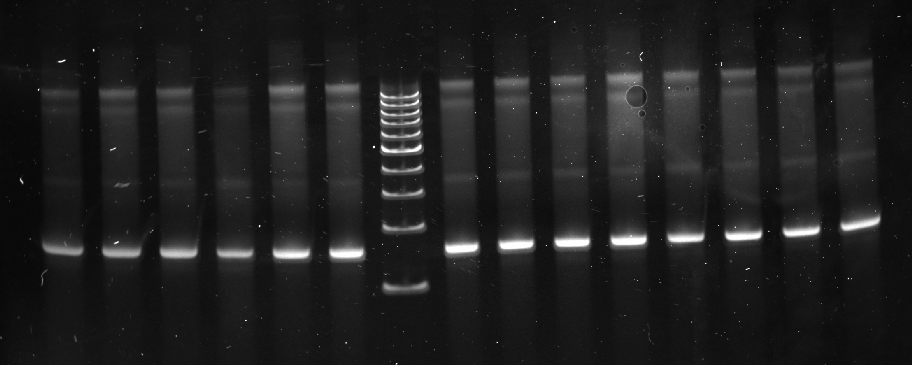
\includegraphics[width=\textwidth]{amplig_a}
    \caption{A}
    \label{fig:amplig_a}
  \end{subfigure}
  \begin{subfigure}[htpb]{0.4\textwidth}
    \centering
    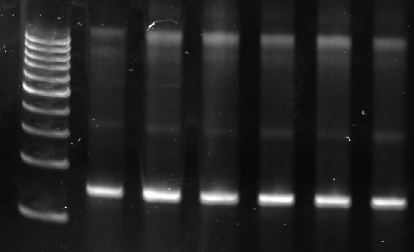
\includegraphics[width=\textwidth]{amplig_b}
    \caption{B}
    \label{fig:amplig_b}
  \end{subfigure}
  \begin{subfigure}[htpb]{0.4\textwidth}
    \centering
    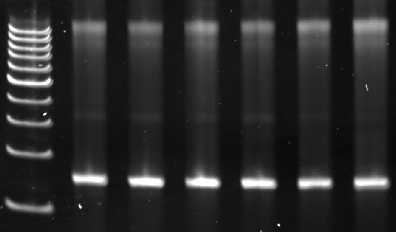
\includegraphics[width=\textwidth]{amplig_c}
    \caption{C}
    \label{fig:amplig_c}
  \end{subfigure}
  \begin{subfigure}[htpb]{0.4\textwidth}
    \centering
    
\includegraphics[width=\textwidth]{test}
    \caption{D}
    \label{fig:amplig_d}
  \end{subfigure}
  \caption{Gel electrophoresis in 8\% TBE gels for (A) amplified lig147 (B) half-C-methylated (C) all-C-methylated, and (D) CpG-methylated DNA. All lanes exhibited a strong band between 100 and 200 nucleotides. Slower-migrating fainter bands corresponded to single-stranded DNA as was expected.}
  \label{fig:amplig}
\end{figure}

\subsection{Nucleosome reconstitution}
\label{ssec:reconstnuc}

EMSA in all cycles yielded strong bands corresponding to naked 147-base pair DNA. It also yielded bands corresponding to reconstituted nucleosomes that are fainter as the proportion of histone octamer decreased in the solution (figure~\ref{fig:reconstnuc}).

\begin{figure}[htpb]
  \centering
  \begin{subfigure}[htpb]{0.4\textwidth}
    \centering
    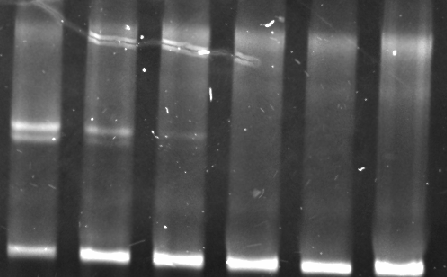
\includegraphics[width=\textwidth]{reconstnuc_a}
    \caption{A}
    \label{fig:reconstnuc_a}
  \end{subfigure}
  \begin{subfigure}[htpb]{0.4\textwidth}
    \centering
    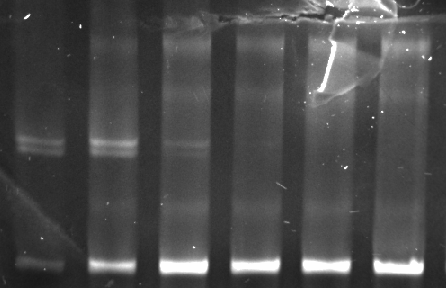
\includegraphics[width=\textwidth]{reconstnuc_b}
    \caption{B}
    \label{fig:reconstnuc_b}
  \end{subfigure}
  \begin{subfigure}[htpb]{0.4\textwidth}
    \centering
    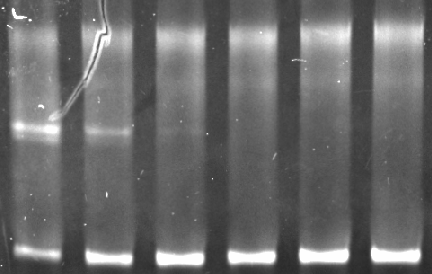
\includegraphics[width=\textwidth]{reconstnuc_c}
    \caption{C}
    \label{fig:reconstnuc_c}
  \end{subfigure}
  \begin{subfigure}[htpb]{0.4\textwidth}
    \centering
    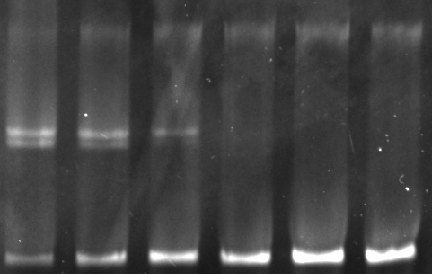
\includegraphics[width=\textwidth]{reconstnuc_d}
    \caption{D}
    \label{fig:reconstnuc_d}
  \end{subfigure}
  \caption{First cycle gel electrophoresis for EMSA in 6\% DNA retardation gels for (A) non-methylated DNA, (B) half-C-methylated (C) all-C-methylated, and (D) CpG-methylated DNA. Lanes for all images (left to right): (1) 1.48:1 histone octamer:DNA, (2) 0.74:1 histone octamer:DNA, (3) 0.37:1 histone octamer:DNA, (4) 0.19:1 histone octamer:DNA, (5) 0.09:1 histone octamer:DNA, and (6) DNA without histone octamer added. These results are representative for all cycles of EMSA SELEX.}
  \label{fig:reconstnuc}
\end{figure}

%% - The sequence preferences of nucleosome 
%% - Disfavored sequences of nucleosome
%% - Methylation effects on nucleosome’s sequence preference

\section{Discussion}
\label{sec:emsaselex_discussion}
%% - The underlying mechanism leading to nucleosome’s sequence preference
%% - Physiological meaning of such preference
%% - Physiological relevance of the methylation effect
%% - A few discussions about Troubleshooting

% I anticipate this to be A LOT shorter

% Debugging should probably be in a separate subsection in the results or discussion section

After the DNA was eluted, barcodes were added using DreamTaq or Phusion (both ThermoFisher) as DNA polymerases.  Gel electrophoresis of the products amplified by DreamTaq yielded bands corresponding to 147 base pairs (figure~\ref{fig:barcoding_a}).  However, gel electrophoresis of the products amplified by Phusion using recommended protocols did not yield this band (figure~\ref{fig:barcoding_b}).

Repeating the Phusion amplification using qPCR yielded saturation curves (figure~\ref{fig:qpcr}), suggesting that amplification indeed took place.  As qPCR required a lower concentration of the template, it was hypothesised that Phusion initially failed because the ligand was too concentrated.  Different DNA polymerases from different vendors are efficient with differing template concentrations – for example, DreamTaq requires ... while Phusion requires ... (citation needed).  Therefore, I diluted the template DNA further by adding \SI{70}{\micro\litre} dilution buffer to each well. The resulting 8\% TBE gel yielded the band corresponding to 147 base pairs (figure~\ref{fig:barcoding_c}), confirming the hypothesis.

\begin{figure}[htpb]
  \centering
  \begin{subfigure}[htpb]{0.4\textwidth}
    \centering
    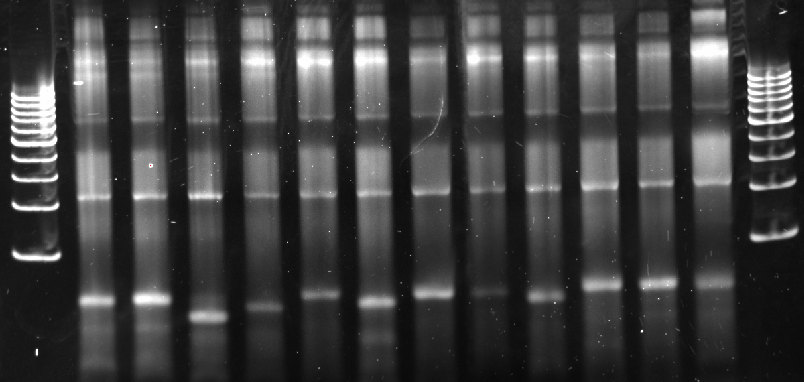
\includegraphics[width=\textwidth]{dreamtaq}
    \caption{A}
    \label{fig:barcoding_a}
  \end{subfigure}
  \begin{subfigure}[htpb]{0.4\textwidth}
    \centering
    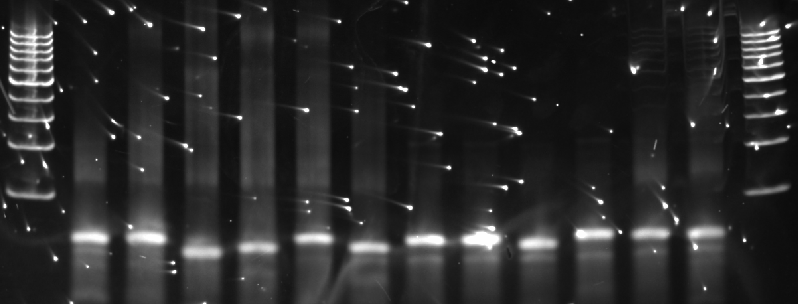
\includegraphics[width=\textwidth]{phusion_old_a}
    \caption{B}
    \label{fig:barcoding_b}
  \end{subfigure}
  \begin{subfigure}[htpb]{0.4\textwidth}
    \centering
    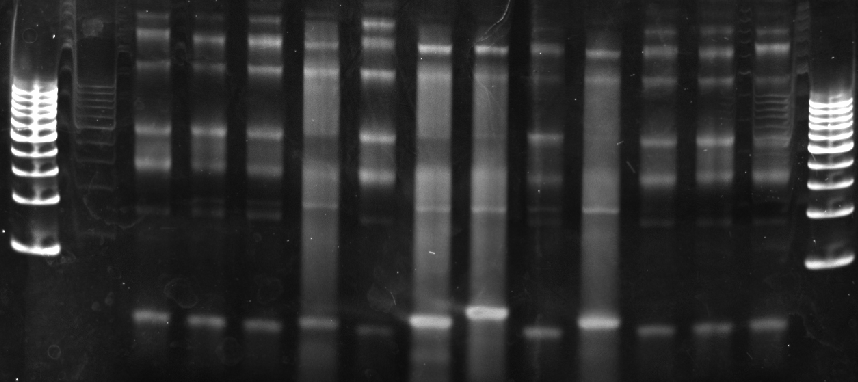
\includegraphics[width=\textwidth]{phusion_new_a}
    \caption{C}
    \label{fig:barcoding_c}
  \end{subfigure}
  \begin{subfigure}[htpb]{0.4\textwidth}
    \centering
    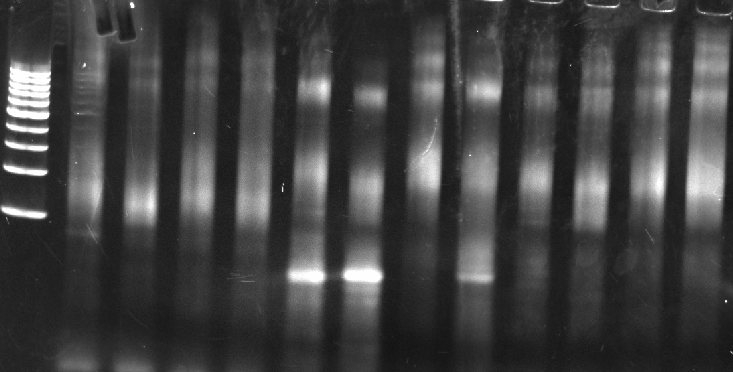
\includegraphics[width=\textwidth]{qpcrgel}
    \caption{D}
    \label{fig:barcoding_d}
  \end{subfigure}
  \caption{A - DreamTaq gel, B - old Phusion gels for rows A and B, C - new Phusion gels for rows A and B, D - qPCR gel}
  \label{fig:barcoding}
\end{figure}

\begin{figure}[htpb]
  \centering
  \begin{subfigure}[htpb]{0.3\textwidth}
    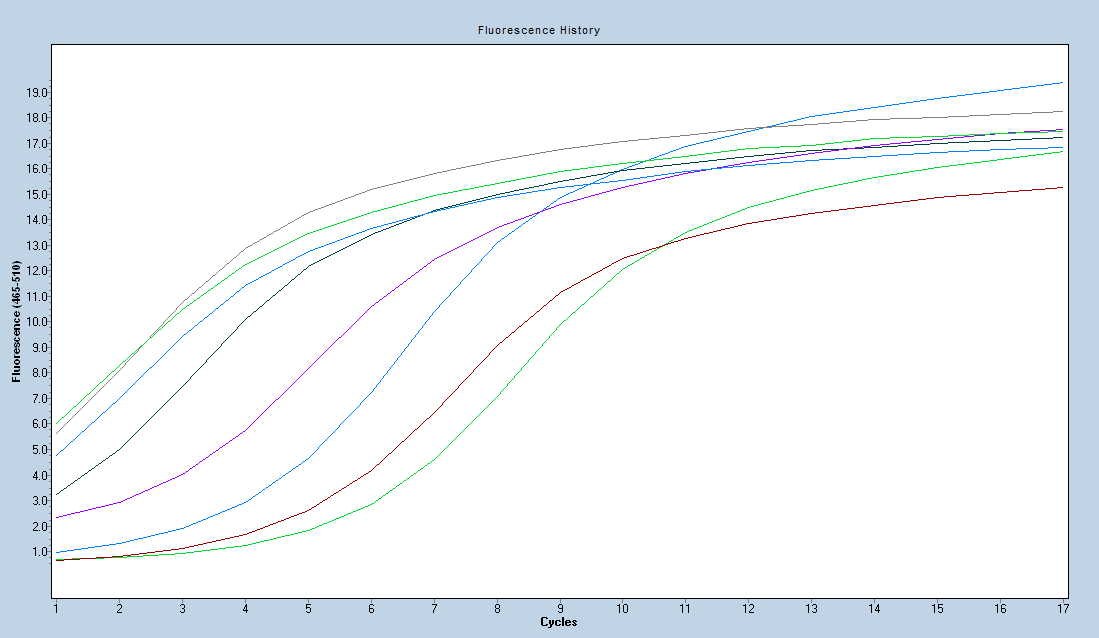
\includegraphics[scale=0.1]{qPCR_B}
    \caption{A}
    \label{fig:qpcr_a}
  \end{subfigure}
  \begin{subfigure}[htpb]{0.3\textwidth}
    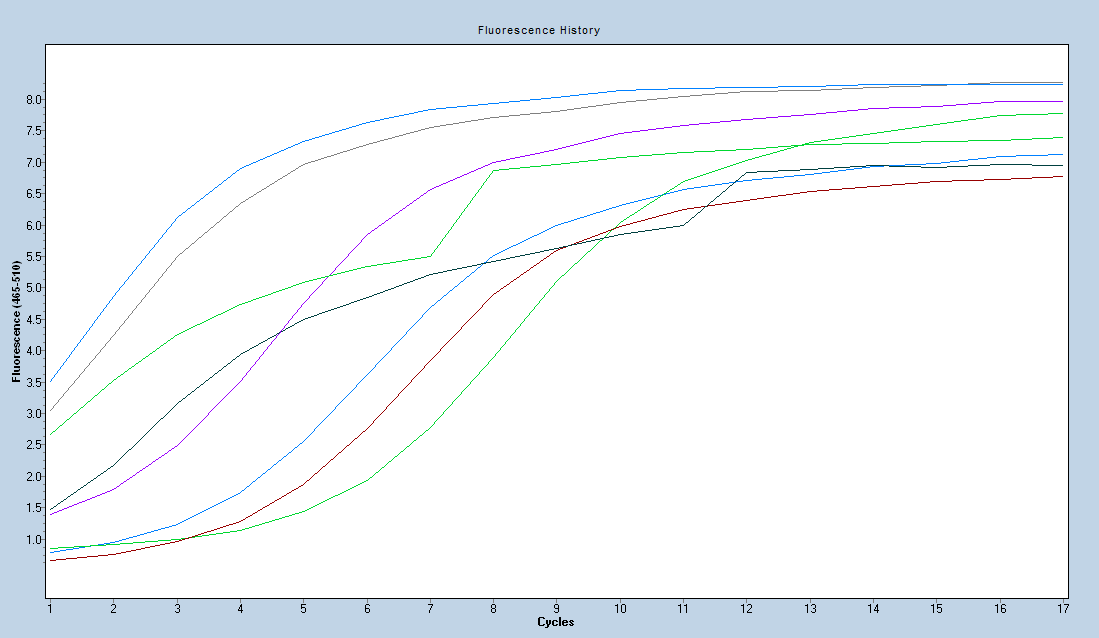
\includegraphics[scale=0.1]{qPCR_D}
    \caption{B}
    \label{fig:qpcr_b}
  \end{subfigure}
  \begin{subfigure}[htpb]{0.3\textwidth}
    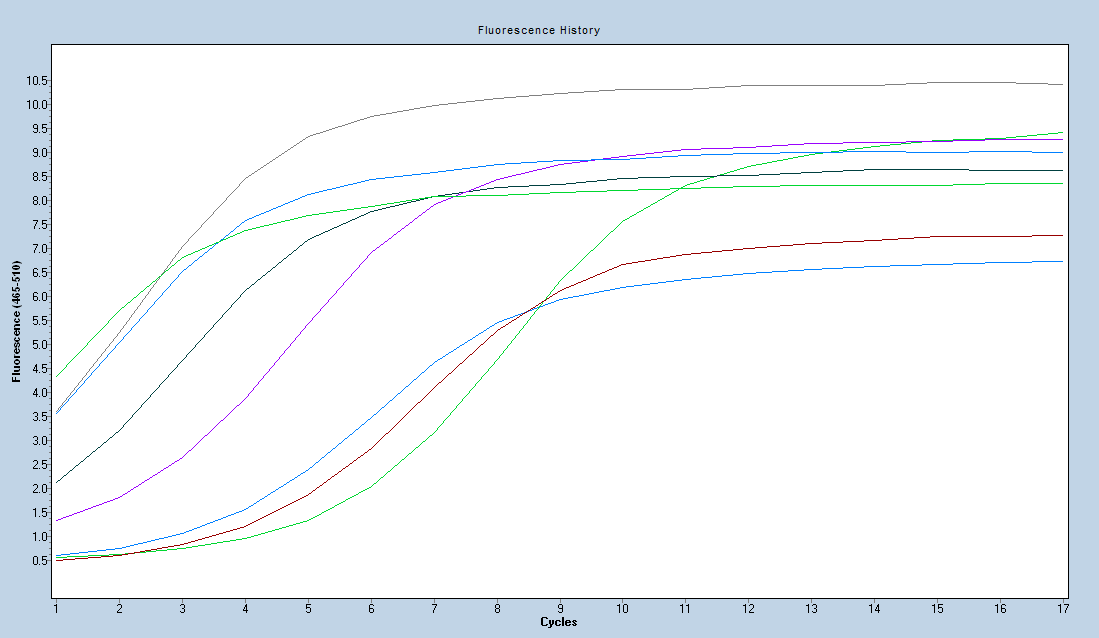
\includegraphics[scale=0.1]{qPCR_F}
    \caption{C}
    \label{fig:qpcr_c}
  \end{subfigure}
  \caption{A - row B, B - row D, C - row H}
  \label{fig:qpcr}
\end{figure}


\chapter{PCR Bias}
\label{ch:pcrbias}

\section{Introduction}
\label{sec:pcrbias_intro}

\subsection{Origin of PCR bias}
\label{ssec:pcrbias_intro_origin}
%% - The origin of PCR bias
% I think I need to find more papers on this

\subsection{How PCR bias affects reliability of sequencing results}
\label{ssec:pcrbias_intro_effects}
%% - How PCR bias affects reliability of sequencing results
% I think I need to find more papers on this
% Olova et al. 2018 mentions DNA methylation, so it will be useful when I'm justifying why I'm adding methylated nucleotides in a step in this project

\subsection{Purpose of study}
\label{ssec:pcrbias_intro_why}
%% - The purpose of this study: provide experiment data, to build a model accounting for such bias, remove such bias in future genomic study

SELEX employs PCR.  Using PCR makes amplified DNA biased towards sequences that are conducive towards PCR amplification, rather than accurately reflect the composition of the heterogenous sample that is amplified. %citation needed
This especially applies when the signal enrichment in the sequencing library is weak.  This is the case for nucleosome-SELEX, where sequence affinities for the nucleosome is weak.

With PCR, sequence biases do not clearly separate DNA sequences bound to nucleosomes from DNA sequences not bound to nucleosomes, as desired.  Instead, both DNA sequences bound to nucleosomes and DNA sequences not bound to nucleosomes have the same bias.  This bias is towards sequences conducive to amplification by PCR.

Here I tested the sequence biases that could be introduced by the choice of DNA polymerase, choice of reagents, cycles of PCR, and purification of DNA after PCR.  This led to constructing a model of PCR bias, which could help users of PCR and SELEX to remove biases to reveal true signals.


\section{Materials and Methods}
\label{sec:pcrbias_methods}
%% - Most parts are the same as the project 1 [just add references to it??]

\subsection{DNA ligand design and preparation}
\label{ssec:pcrbias_methods_lig}

The same input library as \ref{ssec:emsaselex_methods_lig} was used, without methylation.

\subsection{Biases from enzymes}
\label{ssec:pcrbias_methods_enz}

PCR amplification followed manufacturers' specification for the following DNA polymerases: Phire Hot Start II DNA polymerase (ThermoFisher, F122S), Q5 Hot Start High-Fidelity DNA polymerase (New England BioLabs, M0493S), DreamTaq Hot Start DNA Polymerase (ThermoFisher, EP1701), Pfu Turbo DNA Polymerase (Agilent Technologies, 600250), and Phusion High-Fidelity DNA Polymerase (ThermoFisher, F530L).  For each source, DNA was amplified by 4, 8, 12, 16, 20, 24, and 28 cycles.

\subsection{Biases from PCR cycles}
\label{ssec:pcrbias_methods_pcr}

\subsection{Biases from purification}
\label{ssec:pcrbias_methods_pur}

\subsection{Biases from reagent vendors}
\label{ssec:pcrbias_methods_reagent}

\subsection{Sequencing}
\label{ssec:pcrbias_methods_seq}

The same procedures for sequencing as \ref{ssec:emsaselex_methods_seq} were used.

%% - Data analysis

\section{Results}
\label{sec:pcrbias_results}
%% - Different oligonucleotide bias of different PCR enzymes
%% - The variance caused by bottleneck effect 
%% - Dependency of bias on PCR template concentration
%% - Bias caused by reagents from different company
%% - Bias from PCR Purification

\section{Discussion}
\label{sec:pcrbias_discussion}
%% - Relevance of such bias to previous sequencing data
%% - Hints to data analysis in the future 
%% - A few discussions about Troubleshooting

\chapter{Acknowledgements}
\label{ch:ack}

Acknowledgements.

\printbibliography

\end{document}
